% Standalone annotated figure for R2.1 (particle-wall friction = 0 rationale)
%  (a) Full HCA specimen with wedge-marker location
%  (b) Element detail with f^o_{pw_n} (normal) + f^o_{pw_t} (tangential)
%      contact-force arrows at one representative particle–wall contact
%      on the outer cylinder (notation matches Appendix A, Table 3).

\documentclass[border=5pt,tikz]{standalone}
\usepackage{tikz}
\usepackage{graphicx}
\usepackage{amsmath,amssymb}
\usetikzlibrary{positioning, calc, arrows.meta}

\begin{document}

\begin{tikzpicture}[
    every node/.style={font=\small},
]

%% ── Image widths (cm) ──
\def\Wfull{6.0}
\def\Wdet{6.0}
\def\gap{0.5}

%% ── (a) Full HCA ──
\node[anchor=south west, inner sep=0] (full) at (0,0)
  {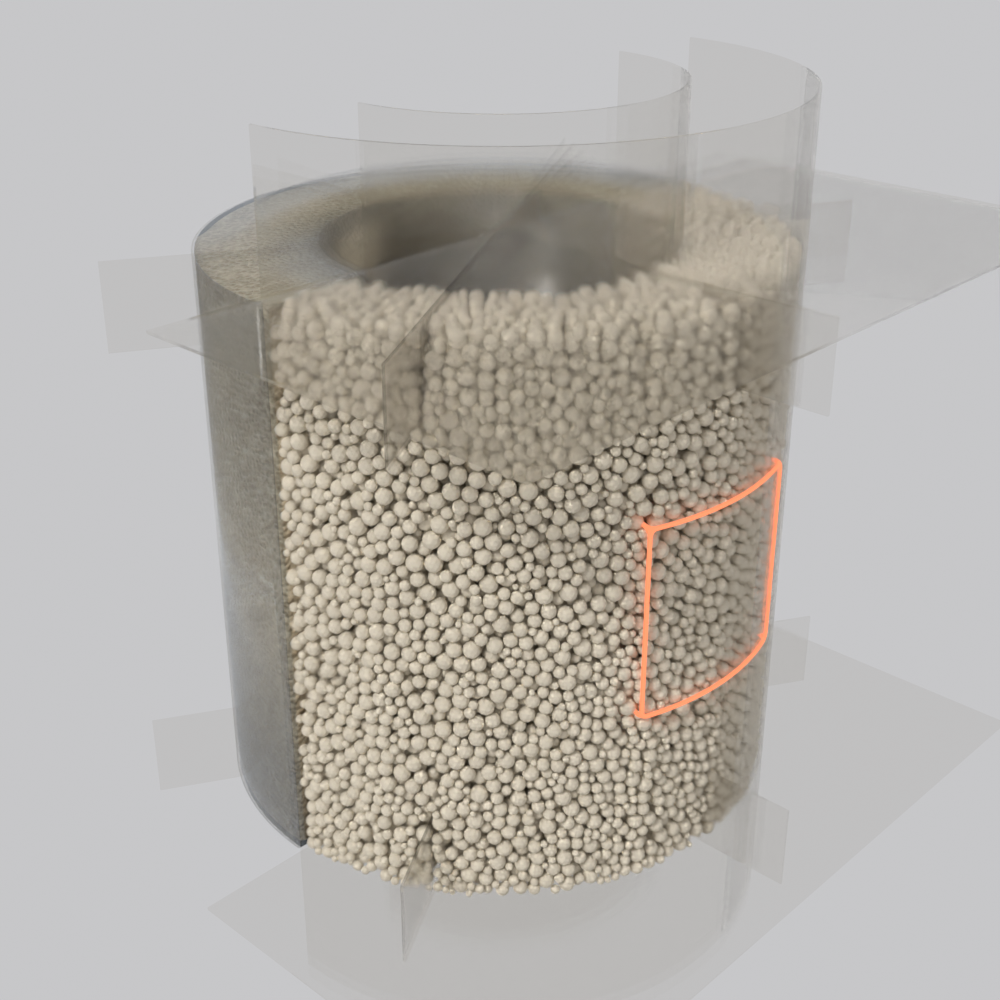
\includegraphics[width=\Wfull cm]{../rcell_full.png}};
\node[below=2pt of full.south] {\textbf{(a)} HCA specimen};

%% ── (b) Detail with force arrows ──
\node[anchor=south west, inner sep=0] (det) at ({\Wfull + \gap},0)
  {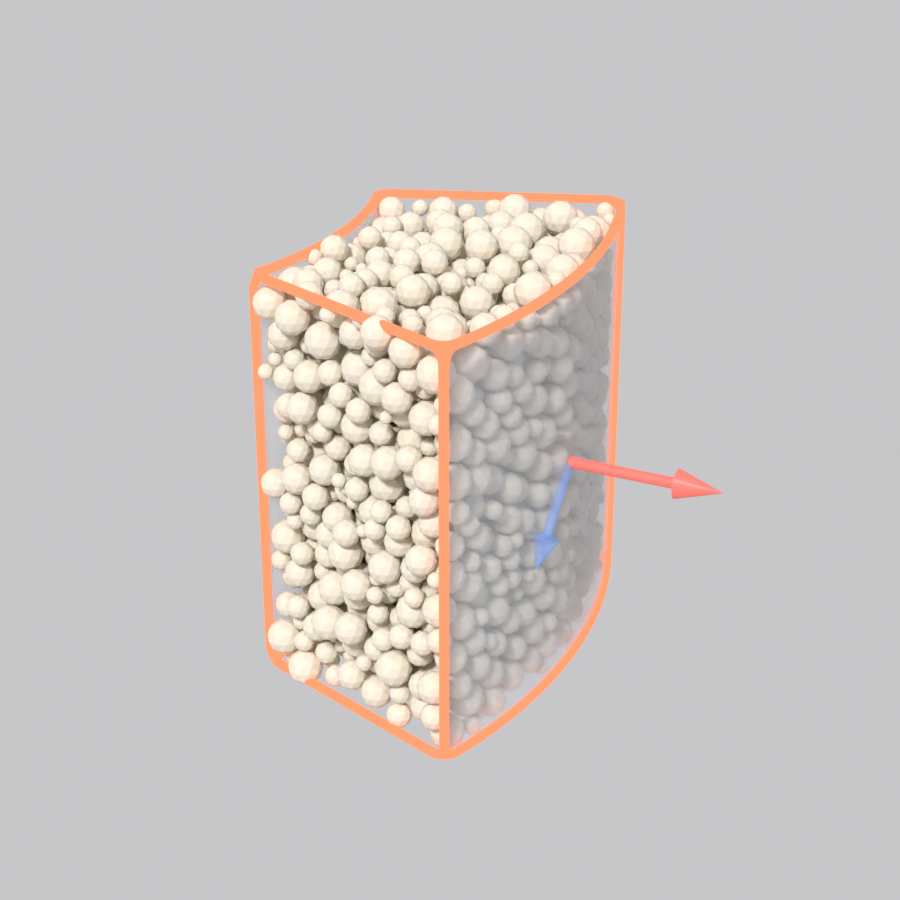
\includegraphics[width=\Wdet cm]{../rcell_detail_forces.png}};
\node[below=2pt of det.south] {\textbf{(b)} Particle--wall contact};

%% ── Connector arrow from wedge-marker on (a) to (b) ──
\coordinate (markA)  at ($(full.south west) + (0.82*\Wfull, 0.46*\Wfull)$);
\coordinate (enterB) at ($(det.south west)  + (0.20*\Wdet, 0.46*\Wdet)$);
\draw[->, very thick, orange!75!black] (markA) -- (enterB);

%% ── Labels for the 3D force arrows on (b) ──
% Head projections (from Blender world_to_camera_view, y measured from TOP):
%   f_n head: (0.8044, 0.5482) → TikZ y-from-bottom ≈ 0.452
%   f_t head: (0.5955, 0.6335) → TikZ y-from-bottom ≈ 0.367
% Labels placed just beyond each head.
\node[font=\footnotesize, red!70!black] at
  ($(det.south west) + (0.86*\Wdet, 0.45*\Wdet)$)
  {$f_{pw_n}^{o}$};
\node[font=\footnotesize, blue!60!black] at
  ($(det.south west) + (0.62*\Wdet, 0.33*\Wdet)$)
  {$f_{pw_t}^{o}$};

\end{tikzpicture}

\end{document}
